\part{Using HPC}
\begin{frame}
\partpage
\end{frame}

\section{Connecting}
\begin{frame}{Basics: Connecting}
\begin{itemize}
\item When connecting to the cluster will we use the SSH secure protocol only.
\item We will use the Linux workstations during this course
\item Please check your workstation is booted into Ubuntu Linux, ask if you need help with this.
\item You are welcome to use your own laptop, however you may need to install some software in order to connect.
\item Later in this section of the slides we will cover the software you may need to install on your own computer.
\end{itemize}
\end{frame}

\subsection{Connecting - SSH}
\begin{frame}{Basics: Connecting}
\begin{itemize}
\item SSH secure protocol only.\hfill\\
\visible<2->{\alert{Supports login, file transfer, remote desktop\ldots}}
\item<3-> HPCS now allows direct access from outside of the CUDN.\hfill\\
\visible<4->{\alert{It is still worth configuring the UIS VPN service\hfill\\
\qquad http://www.ucs.cam.ac.uk/vpn}}\hfill\\
\visible<5->{\qquad\alert{Useful for other CUDN only services.}}
\end{itemize}
\end{frame}

\subsection{Login Nodes}
\begin{frame}{Basics: Connecting}
\begin{itemize}
\item To access the Peta4-Skylake (CPU cluster) nodes:\hfill\\
ssh \textless username\textgreater @login-cpu.hpc.cam.ac.uk
\item To access the Peta4-KNL (KNL cluster) nodes:\hfill\\
ssh \textless username\textgreater @login-knl.hpc.cam.ac.uk
\item To access the Wilkes2-GPU (GPU cluster) nodes:\hfill\\
ssh \textless username\textgreater @login-gpu.hpc.cam.ac.uk
\end{itemize}
\end{frame}

\subsection{Linux Clients}
\begin{frame}{Connecting: Linux Clients}
\begin{itemize}
\item {\color<2->{red}ssh}, scp, sftp, {\color<2->{red}rsync}\hfill\\
\alert{\small Installed (or installable), in Ubuntu we will use 'Terminal'.}
\item {X Windows, for using graphical applications remotely}
\alert{\small This is already installed on your desktop.}
\end{itemize}
\end{frame}

\subsection{Login}
\begin{frame}{Connecting: Login}
\begin{itemize}
\item From Linux/MacOSX/UNIX (or Cygwin):\hfill\\
\alert{ssh -Y \textbf{abc123}@login-cpu.hpc.cam.ac.uk}
\pause
\item From graphical clients:\hfill\\
Host: \alert{login-cpu.hpc.cam.ac.uk}\hfill\\
Username: \alert{\textbf{abc123}} (your UCAM account name)
\pause
\item login-cpu.hpc will map to a random login node\hfill\\
\alert{i.e. one of login-e-9,\ldots\,, login-e-16}\hfill\\
\uncover<4->{{\color{red}NB you'll never connect to the head node.}}
%\item<5->Similarly for other systems (e.g.\ cardio-login.hpc, login-mrc-bsu.hpc,\ldots). 
\end{itemize}
\end{frame}

\subsection{First time login}
\begin{frame}{Connecting: First time login}
\begin{itemize}
\item{The first connection to a particular hostname produces the following:}
\begin{semiverbatim}\footnotesize
The authenticity of host 'login-e-10.hpc.cam.ac.uk  (128.232.224.47)' can't be established.

RSA key fingerprint is

{\color<2->{red}0b:ef:59:90:fb:13:4a:c9:56:82:7b:cd:4b:2b:e1:3b}.

Are you sure you want to continue connecting (yes/no)? {\color<3->{red}yes}

Warning: Permanently added 'login-sand2.hpc.cam.ac.uk' (RSA) to the list of known hosts.
\end{semiverbatim}
\smallskip\item{\alert{One should always check the fingerprint before typing ``yes''.}}
\item{Graphical SSH clients \emph{should} ask a similar question.}
\item{Designed to detect fraudulent servers.}
\end{itemize}
\end{frame}

\begin{frame}[fragile]{Connecting: First time login}
\begin{itemize}
\item{You may be presented with any of the following fingerprints (depending on your client):}
\begin{semiverbatim}\footnotesize

MD5:0b:ef:59:90:fb:13:4a:c9:56:82:7b:cd:4b:2b:e1:3b
SHA256:sSkVfzpwjwiFvxLcdPoDpN8IsN3kt0ZSywhDhPKZPAg

MD5:34:9b:f2:d2:c6:b3:5c:63:99:b7:27:da:5b:c8:16:fe
SHA256:HsiY1Oe0M8tS6JwR76PeQQA/VB7r8675BzG5OYQ4h34

MD5:64:7c:7c:ff:05:9d:0e:dc:06:fe:f1:c2:10:37:7a:85
SHA256:wq9ljBfPa7lXXpQq+rk5JTBXLJO/kXjOc5A7rp4ENzA

\end{semiverbatim}
\end{itemize}
\end{frame}

\subsection{File Transfer with rsync: an example}
\begin{frame}{Connecting: File Transfer}
\begin{itemize}
\item From Linux/MacOSX/UNIX (or Cygwin):\hfill\\
\alert{\footnotesize rsync -av \textbf{old\_directory/} abc123@login.hpc.cam.ac.uk:/home/abc123/new\_directory}\hfill\\
copies contents of old\_directory to $\tilde{}\text{/home/abc123/new\_directory}$.\hfill\\\smallskip
\pause
\alert{\footnotesize rsync -av \textbf{old\_directory} abc123@login.hpc.cam.ac.uk:/home/abc123/new\_directory}\hfill\\
copies old\_directory (and contents) to $\tilde{}\text{/home/abc123/new\_directory/old\_directory}$.\hfill\\
\pause
\item[$\ast$]For transfers in the opposite direction, place the remote machine as the first argument.
\end{itemize}
\end{frame}
%
\section{Connecting from other clients}
\begin{frame}{Basics: Connecting from other clients}
\begin{itemize}
\item{When using your own computer you you may need to install some software in order to connect.}
\pause
\item{There are quite a few choices of software packages for this, we will just cover a few.}
\pause
\item{Our website \url{https://www.csd3.cam.ac.uk/using-clusters/connecting} covers this in more detail.}
\end{itemize}
\end{frame}

\subsection{MacOSX}
\begin{frame}{Connecting: MacOSX/UNIX Clients}
\begin{itemize}
\item {\color<2->{red}ssh}, scp, sftp, {\color<2->{red}rsync}\hfill\\
\alert{\small Installed (or installable) OS X has a native terminal package. This can be launched by clicking Apple \textgreater Go \textgreater Utilities and then clicking the Terminal icon.}
\item<3-> TurboVNC \alert{\small (for remote desktop, 3D optional)}\hfill\\
\alert{\small http://sourceforge.net/projects/turbovnc/files/}
\item<4-> On MacOSX, install \alert{XQuartz} to display remote graphical applications.\hfill\\
\alert{\small http://xquartz.macosforge.org/landing/}
\end{itemize}
\end{frame}

\subsection{Windows Clients}
\begin{frame}{Connecting: Windows Clients}
\begin{itemize}
\item<1-5> putty, pscp, psftp\hfill\\
\alert{\small http://www.chiark.greenend.org.uk/~sgtatham/putty/download.html}
\item<2-5> WinSCP\hfill\\
\alert{\small http://winscp.net/eng/download.php}
\item<3-5> TurboVNC \alert{\small (remote desktop, 3D optional)}\hfill\\
\alert{\small http://sourceforge.net/projects/turbovnc/files/}
\item<4-5> Cygwin \visible<5>{\alert{\small (provides an application environment similar to Linux)}}\hfill\\
\alert{\small http://cygwin.com/install.html}\hfill\\
\visible<5>{\alert{\small Includes X server for displaying graphical applications running remotely.}}
\item<6> MobaXterm\hfill\\
\alert{\small http://mobaxterm.mobatek.net/}
\end{itemize}
\end{frame}

\subsection{Windows Users}
\begin{frame}{MobaXterm SSH (Windows)}
\begin{center}
\centerline{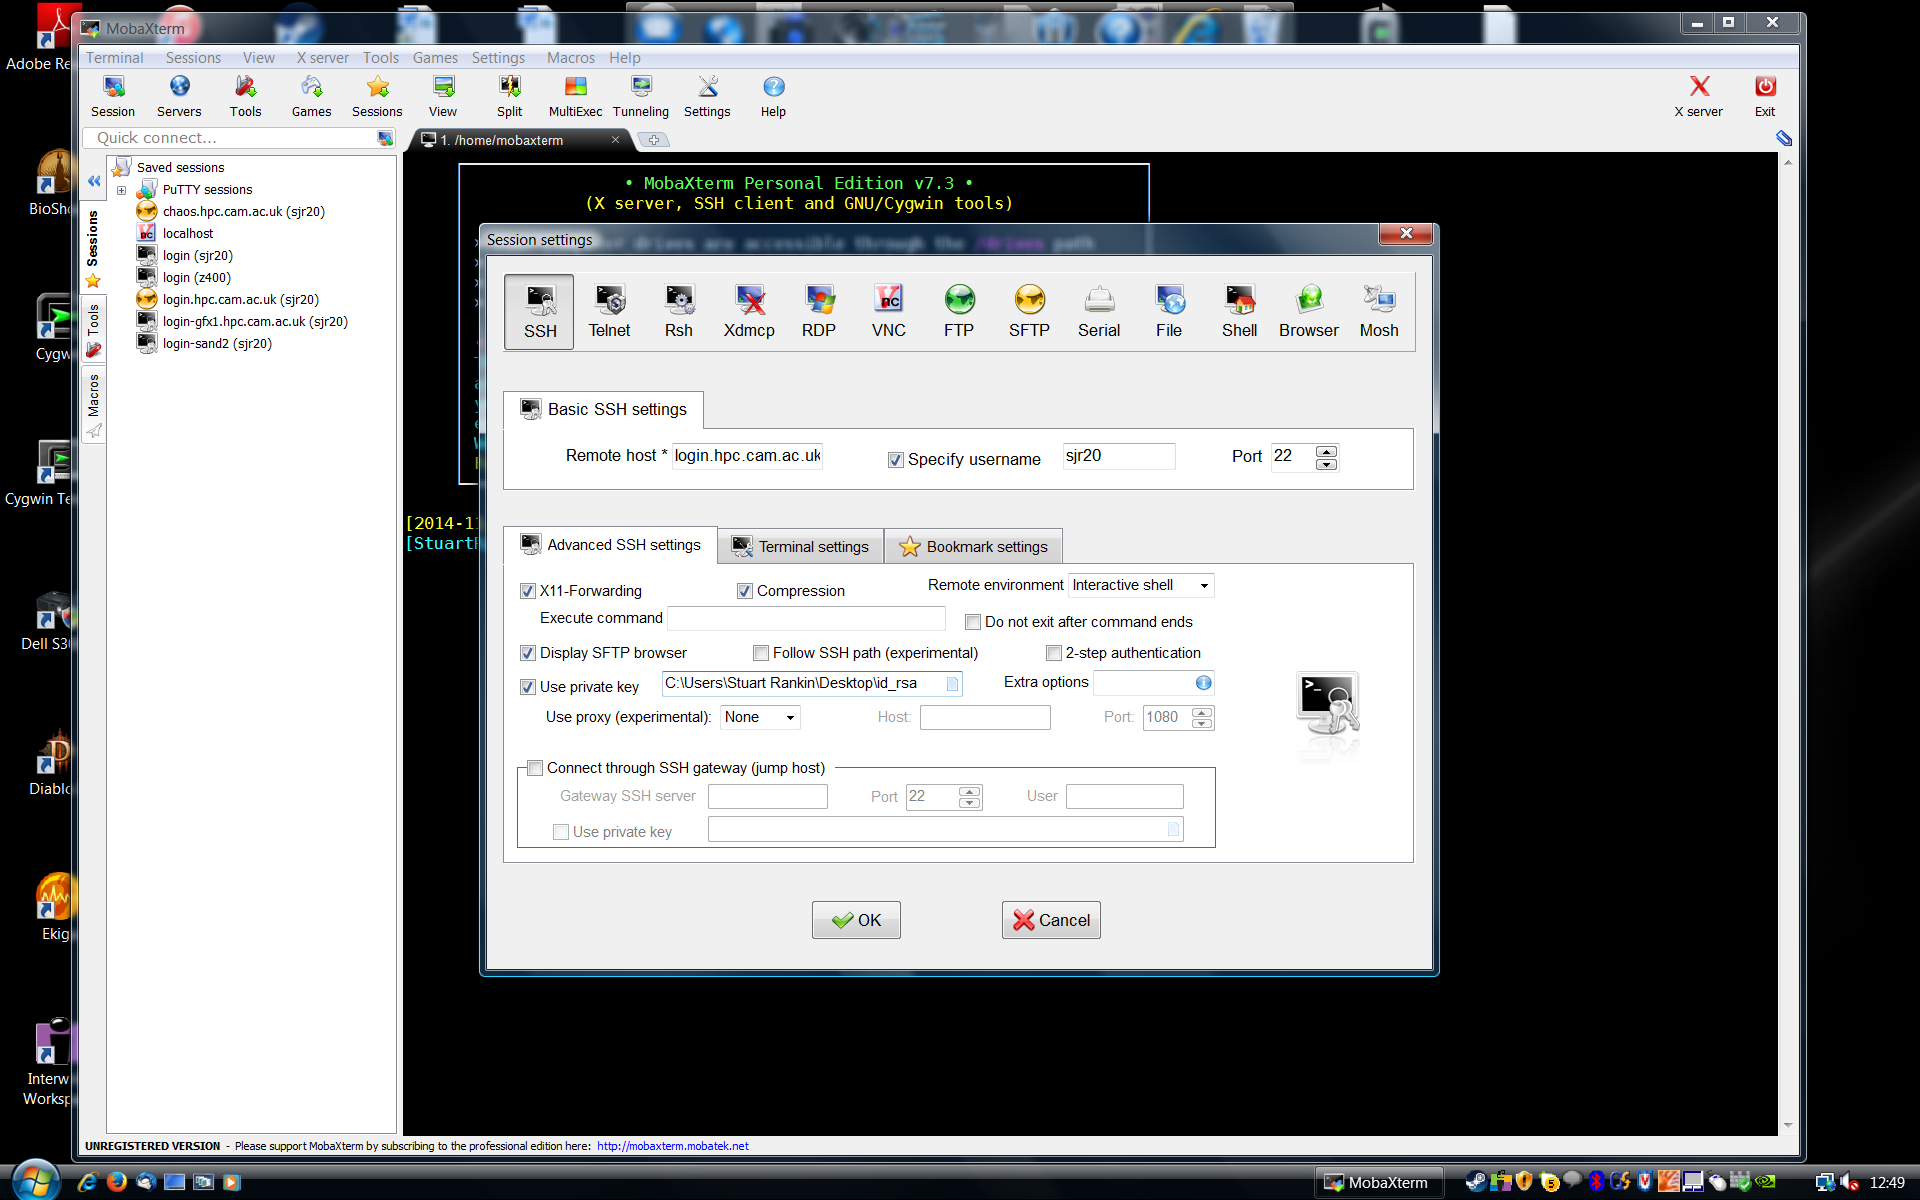
\includegraphics[height=0.8\textheight]{imgs/mobaxterm-SSH-settings2.png}}
\end{center}
\end{frame}

\begin{frame}{MobaXterm SSH (Windows)}
\begin{center}
\centerline{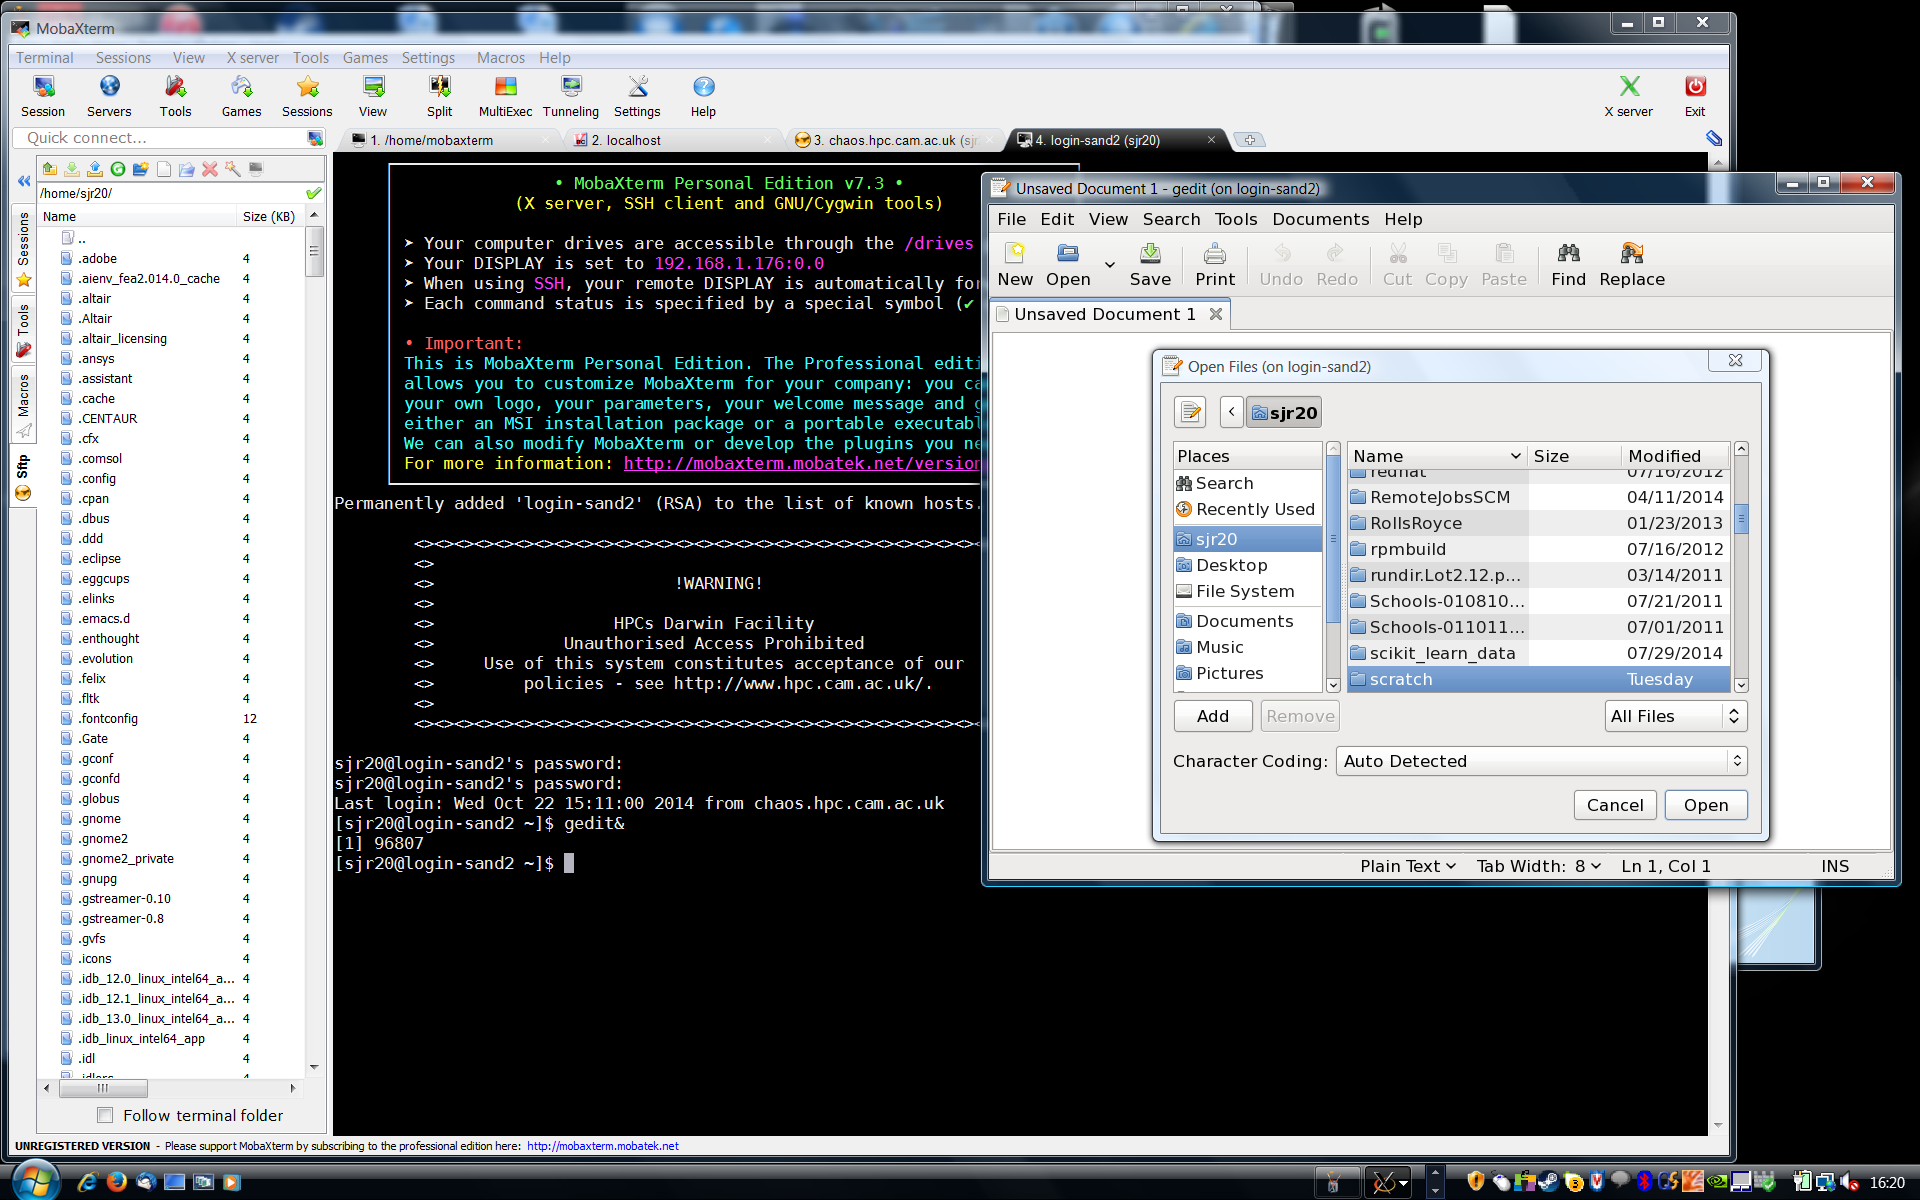
\includegraphics[height=0.8\textheight]{imgs/mobaxterm-SSH-session.png}}
\end{center}
\end{frame}

\section{Simple command line operations}
\begin{frame}{Simple command line operations}
\begin{itemize}
\item{Some simple exercises will help us gauge your experience.}
\item{Exercise 1: Login with SSH}
\item{Exercise 2: SFTP file transfer}
\item{Excecise 3: Learn more about a command}
\item{Exercise 4: Unzip the excercises.tar file}
\item{Excecise 5: Navigating the command line}
\end{itemize}
\end{frame}

\subsection{Exercise 1: Login with SSH}
\begin{frame}{Exercise 1: Login}
Using a Linux terminal you will login to the cluster with your HPC training account.
\begin{itemize}
\item{Start the terminal by double clicking on the terminal icon}
\item In your terminal enter:
\item{ssh -Y \textbf{abc123}@login-cpu.hpc.cam.ac.uk}\\
Replace abc123 with your training account username 
\item {Enter your password as supplied on the sheet}
\item{Leave this terminal open, you will need it for exercise 3!}
\end{itemize}
\end{frame}

\subsection{Exercise 2: SFTP file transfer - pt1}
\begin{frame}{Exercise 2: Transfer some files}
You will need to transfer the exercise files to the cluster.
\begin{itemize}
\item{Open a second Linux terminal on your training computer.}
\item{Enter this command: cd \alert{\footnotesize \path{~\Course_material}}}
\item{Check the file 'exercises.tar is in your directory listing}
\item{Hint: ls}
\end{itemize}
\end{frame}

\subsection{Exercise 2: SFTP file transfer - pt2}
\begin{frame}{Exercise 2: Transfer some files}
Transfer the exercises.tar to your HPC home folder.
\begin{itemize}
\item{In the local terminal on your training computer enter the command:}
\item \alert{\footnotesize sftp abc123@login-cpu.hpc.cam.ac.uk}\\
Change abc123 to your training account username
\item{The command: \alert{\footnotesize put exercises.tar} will transfer the file from your local computer to the remote one}
\item{Check the file 'exercises.tar is in your directory listing}
\item{Hint: ls}
\item Type 'exit' to close the local terminal
\end{itemize}
\end{frame}

\subsection{Excercise 3: Learn more about a command}
\begin{frame}{Exercise 3: Learn more about a command}
\begin{itemize}
\item[(a)]{View the man page for the \alert{cp} command by doing \alert{man cp}. 
Use \alert{SPACE} to page down and \alert{b} to page up. Press \alert{q} to exit the manual page command.}
\item[(b)]{View the man pages for the \alert{mkdir} and \alert{mv} commands. }
\end{itemize}
\end{frame}

\subsection{Excercise 4: Unzip the excercises.tar file}
\begin{frame}{Exercise 4: Unzip the excercises.tar file}
  \begin{itemize}

\item[(a)]{Use the \alert{ls} to list your home folder contents --- you should see the copy of exercises.tar.}
 \visible<3->{\begin{description}
\item[\emph{Hints:}]{Do \alert{cd\quad$\tilde{}$} then \alert{ls -al}. Note that \alert{cd\quad$\tilde{}$} will take you back to your home directory.}
\end{description}}

\item[(b)]{Unpack the tar archive to create an exercise subdirectory.}
\visible<4->{\begin{description}
\item[\emph{Hints:}]{Do \alert{tar -xvf exercises.tar}}
\end{description}}
\item[(c)]{Move the exercise subdirectory to a new directory.}
\visible<4->{\begin{description}
\item[\emph{Hints:}]{Do \alert{mv -Rf exercises myexercises}}
\end{description}}
\end{itemize}
\end{frame}

\subsection{Excercise 5: Navigating the command line}
\begin{frame}{Exercise 5: File listings}
\begin{itemize}

\item[(a)]{In a terminal logged into the cluster list the contents of your current directory \alert{ls}. This won't show everything --- use \alert{ls -al} for a long listing showing all files. Initially you will start in your home directory --- use \alert{pwd} to print the name of your current working directory. If you get lost, you can always do \alert{cd} without arguments to return to your home directory.}

\item[(b)]{Focus your long listing on \alert{all files with names beginning ``myexercises''}.}
 \visible<2->{\begin{description}
\item[\emph{Hints:}]{Do \alert{ls -al myexercises*}}
\end{description}}

\item[(c)]{Print a long listing of the subdirectory \alert{myexercises}.}
 \visible<3->{\begin{description}
\item[\emph{Hints:}]{Do \alert{ls -al myexercises/}.}
 \end{description}}

\end{itemize}
\end{frame}








